\documentclass[lettersize,journal]{IEEEtran}
\usepackage{amsmath,amsfonts}
\usepackage{algorithmic}
\usepackage{algorithm}
\usepackage{array}
\usepackage[caption=false,font=normalsize,labelfont=sf,textfont=sf]{subfig}
\usepackage{textcomp}
\usepackage{stfloats}
\usepackage{url}
\usepackage{verbatim}
\usepackage{graphicx}
\usepackage{cite}
\usepackage{longtable} % for tables
\usepackage{booktabs} % for tables

\hyphenation{op-tical net-works}
\setlength{\parindent}{0pt}

\begin{document}

\title{Neural Networks-Deep Learning \\ 3rd Assignment}
\author{Papadakis Konstantinos Fotios}
% The paper headers
\markboth{Neural Networks-Deep Learning, 3rd Assignment, 2024}
\maketitle

\begin{abstract}
This is the third Assignment of the course "Neural Networks-Deep Learning". It expands our 
knowledge on neural networks by creating an transformer neural network which is trained on 
the MNIST dataset. The network takes as input an image from the dataset and returns an image
depicting the next image in the sequence, as generated by the transformer itself.  
\end{abstract}

\section{Introduction}
\subsection{Dataset}
Reflecting on the higher complexity of the task at hand we have chosen to work with a simpler
dataset this time. The MNIST dataset is a collection of 70.000 images of handwritten digits,
each of which is $28 \times 28$ pixels in size. The dataset is split in 60.000 training images and
10.000 test images. Here is a sample of the dataset:
\begin{figure}[H]   
    \centering
    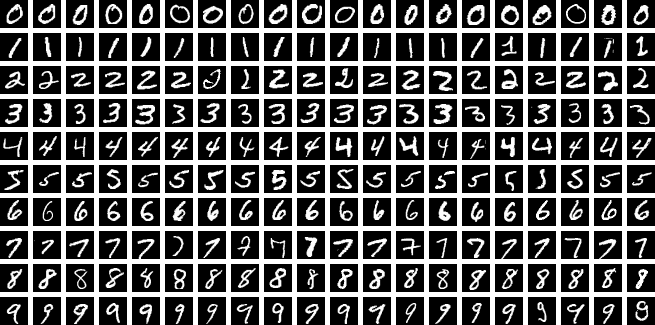
\includegraphics[width=0.5\textwidth]{media/MNIST_dataset_example.png}
    \caption{Sample of the MNIST dataset}
\end{figure}

\subsection{Transformers}
A transformer is a neural network architecture which is based on the multi-head attention
mechanism, where attention is a machine learning method that determines the importance of
each component relative to the the other components in a sequence. This architecture was 
first introduced in the paper "Attention is All You Need" by Vaswani et al. in 2017.

\smallskip

A transformer network is typically composed of an encoder and a decoder. The key components
of the architecture as mentioned in the paper are:
\begin{itemize}
    \item \textbf{Word Embeddings}: The words are represented as vectors in a high-dimensional space.

    \item \textbf{Positional-Encoding}: To differentiate sentences with the same words but in different
    word order, positional encoding is used. During that process we represent the relative position of 
    the words in the sentence with a fixed-size vector. 

    \item \textbf{Multi-Head Self-Attention Mechanism}: In a self-attention mechanism we generate 
    queries (Q), keys (K) and values (V) for each input sequence instructing the model to focus on
    different parts of the input sequence when generating the output. The multi-head mechanism is an
    extension of the self-attention mechanism that allows the model to capture different aspects of the
    input sequence by creating multiple parallel attention heads.

    \item \textbf{Encoder-Decoder Attention}: The encoder focuses on extracting meaningful 
    and compressed representations (latent vectors) of the input. The decoder can decide which 
    parts of the input sequence are most relevant, generating the output. 

    \item \textbf{Residual Connections}: Allow each sub-unit, like the multi-head attention mechanism,
    to focus on solving only one part of the problem. Retains previous self-attention, word and positional
    encoding to allow the encoder-decoder attention to focus on the relevant parts of the input sequence.

    \item \textbf{Feed-Forward Neural Network}: It consists of two linear transformations with a ReLU 
    activation function in between.
\end{itemize}

% simple_transformer.py
\section{Simple Transformer Neural Network}
The first approach we implement revolves around a CNN encoder and a CNN decoder. 
Here are the specific roles of each component:
\begin{itemize}
    \item \textbf{Encoder}: The encoder extracts a latent representation of the input image, which is 
    a lower-dimensional representation of that image.
    \item \textbf{Transformer}: The transformer modifies that representation to approximate 
    the next image in the sequence.
    \item \textbf{Decoder}: The decoder takes the modified representation and generates an
    image from it.
\end{itemize}
The code itself can be sufficiently described by the following steps:
\begin{itemize}
    \item \textbf{MNISTSequenceDataset Class:} Here we create a dictionary with the keys being the 
    the digits zero through nine and the values being the indices of the images in the MNIST dataset.
    When retrieving an item from the dataset we get back the current image and a random image of the 
    next digit.
    \item \textbf{CNNEncoder Class:} The encoder is a simple convolutional neural network with two
    convolutional layers, two ReLU activation functions a flatten layer and a linear layer. It compresses
    the input image into a latent representation. It forwards the latent representation itself.
    \item \textbf{Transformer Class:} The transformer is a simple neural network with two linear layers
    and a ReLU activation function. It forwards the modified latent representation.
    \item \textbf{CNNDecoder Class:} The decoder is a simple convolutional neural network with 
    a fully connected layer which receives the latent vector, two transposed convolutional layers and 
    two activation functions (one ReLU and one tanh). It forwards the generated image.
    \item \textbf{MNISTSequencePredictor Class:} The predictor is the class of the program which brings
    together the encoder, the transformer and the decoder. It encodes the current image, transforms it
    and decodes the next image in the sequence. It is the one that helps us visualize the results too.
    \item \textbf{Training Loop:} We move the model MNISTSequencePredictor() to our computational device
    and train as we have done on the last two assignments. Two important notes are that we use the Mean 
    Squared Error loss function and the Adam optimizer with a learning rate of 0.001.
\end{itemize}
Here are some samples of the images generated by the simple transformer network:
\begin{figure}[H]   
    \centering
    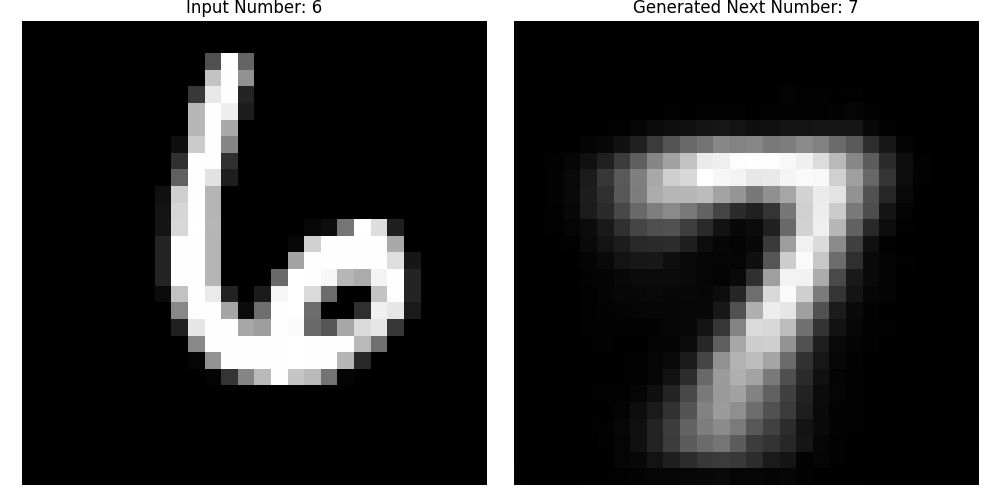
\includegraphics[width=0.5\textwidth]{media/Figure_1.png}
    \caption{Figure 1}
\end{figure}
\begin{figure}[H]   
    \centering
    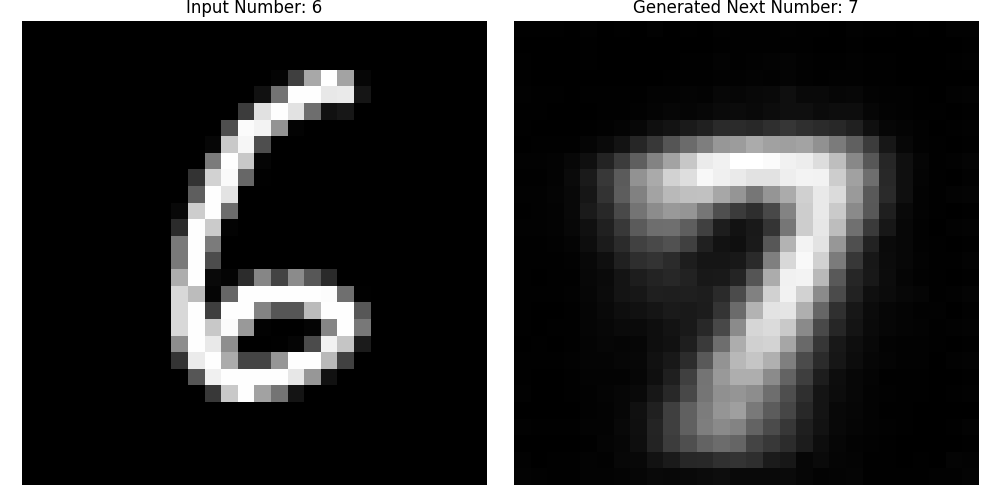
\includegraphics[width=0.5\textwidth]{media/Figure_2.png}
    \caption{Figure 2} 
\end{figure}
\begin{figure}[H]   
    \centering
    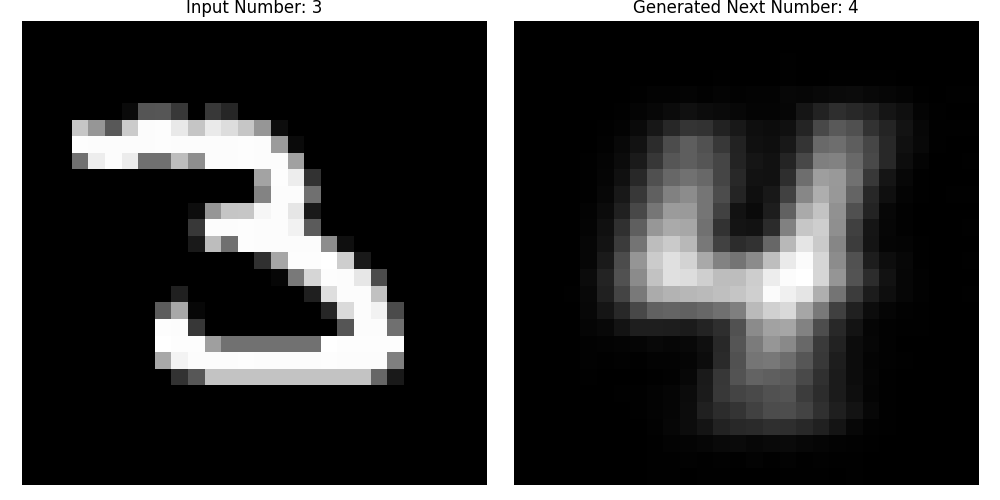
\includegraphics[width=0.5\textwidth]{media/Figure_3.png}
    \caption{Figure 3}
\end{figure}
\begin{figure}[H]   
    \centering
    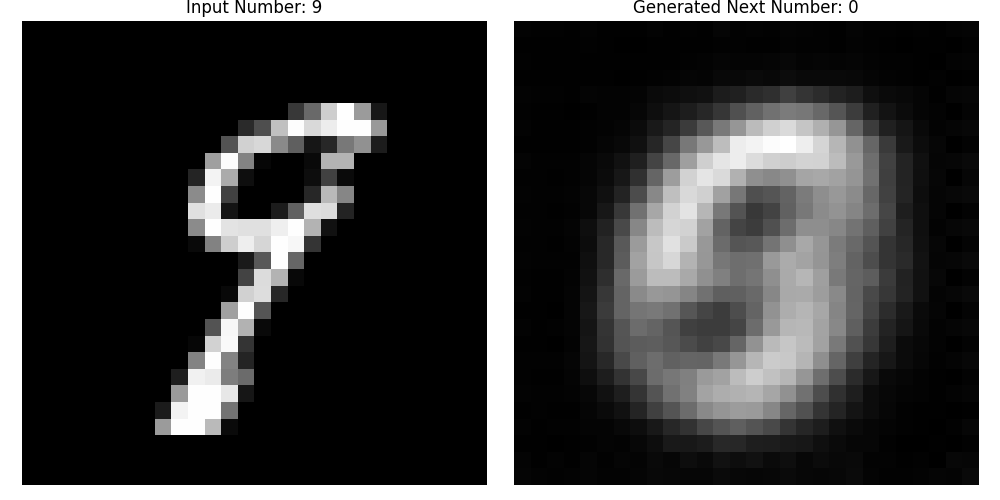
\includegraphics[width=0.5\textwidth]{media/Figure_4.png}
    \caption{Figure 4}
\end{figure}

%self_attention_transformer.py
\section{Self-Attention Transformer Neural Network}
Now we set out to incorporate the self-attention mechanism in our transformer network. It is an 
important part of the transformer architecture, as it allows the network to focus on different
parts of the input sequence when generating the output. As we omitted it in the previous algorithm,
we implement it on this second approach. The extra functionality is the \textbf{Self-Attention mechanism} 
which allows the model to capture different aspects of the input sequence by creating multiple parallel 
attention heads.\\
In code this change shows up as follows:
\begin{itemize}
    \item \textbf{Init Function:}
    \begin{itemize}
        \item 128 is the dimension of the latent space.
        \item 4 is the number of attention heads.
        \item We create a multi-head attention layer with 128 dimensions and 4 heads.
        \item We create a feed-forward neural network with two linear layers and a ReLU activation function.
        \item We create two normalization layers to improve the training process.
    \end{itemize}
    \item \textbf{Forward Function:}
    \begin{itemize}
        \item We first take the input
        \item We pass it through the multi-head attention layer
        \item We add the input to the output of the multi-head attention layer
        \item We pass the result through the normalization layer
        \item We pass the result through the feed-forward neural network
    \end{itemize}
\end{itemize}

\section{Transformer Networks Comparison}
The two transformers manage to achieve similarly high accuracy rates and the images they generate
are of identical quality. Here are the results:
\begin{itemize}
    \item \textbf{Simple Transformer}: Accuracy = , Loss = 
    \item \textbf{Self-Attention Transformer}: Accuracy = 86.63\%, Loss = 0.2363 
\end{itemize}
\begin{figure}[H]   
    \centering
    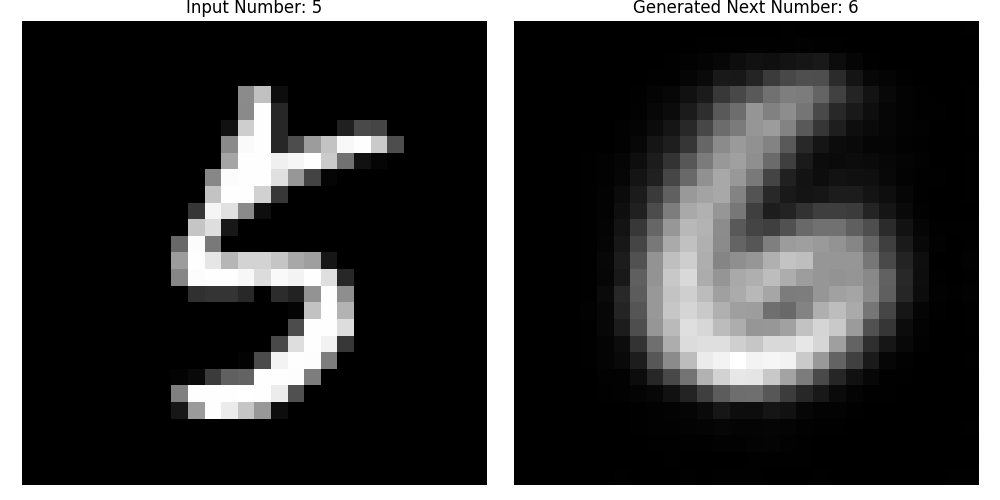
\includegraphics[width=0.5\textwidth]{media/Simple.png}
    \caption{Simple Transformer}
\end{figure}
\begin{figure}[H]   
    \centering
    \includegraphics[width=0.5\textwidth]{media/Self_Attention.png}
    \caption{Self-Attention Transformer}
\end{figure}

% pca_reconstruction.py
\section{PCA}
PCA (Principal Component Analysis) is dimensionality reduction technique that we used in order to
reduce the $28 \times 28 = 784$ dimensions into 50 principle components. The purpose of experimenting 
with it is to cross-reference the resulting images with the ones produced by the transformer network.\\
The PCA code is based on the following logic:
\begin{itemize}
    \item \textbf{Normalize}: Normalize the pixel values of the MNIST dataset to the range [0, 1] by
    dividing by 255.
    \item \textbf{Apply PCA}: Reduce the dimensionality of the dataset from 784 to 50 principal components.
    This means projecting the 784-dimensional data into a 50-dimensional space.
    \item \textbf{Select Digit}: Choose a digit from the transformed dataset to generate a new digit.
    \item \textbf{Perturbation}: Add a small random noise to the selected digit in the PCA space. The 
    noise is just added to the PCA reduced digit. 
    \item \textbf{Inverse Transform}: Transform the perturbed digit back to the original dimensions.
    \item \textbf{Visualization}: Visualize both the original and the generated digits for comparison.
\end{itemize}
The images generated from the PCA algorithm exhibit rough transitions on space that should be empty.
This phenomenon is explained by the low dimensions which we attempted to contain the a lot larger 
dimensionality of the original dataset. Here is a gradual increase in the number of principal components
used in the PCA algorithm which results in better clarity:
\begin{figure}[H]   
    \centering
    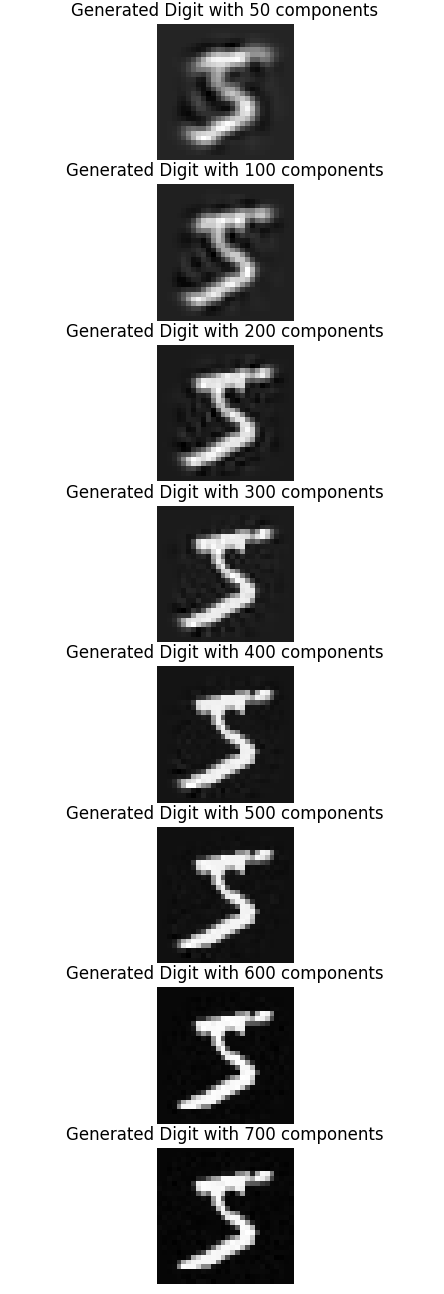
\includegraphics[width=0.4\textwidth]{media/PCA_components.png}
    \caption{PCA Reconstruction}
\end{figure}

% addition_transformer.py
% \section{Addition Transformer}
% As an additional challenge we were encouraged to also use the transformer to portray the sum
% of two numbers taken from the MNIST dataset.

% cnn_interpreter.py and generate_images.py
\section{CNN Interpreter}
As an attempt to prove that the transformer generated images good enough to be recognized by a 
neural network, we train the CNN on both the MNIST dataset and our custom dataset comprised of
transformer generated images. To generate the images we will utilize a version of the simple
transformer where the output isn't a presentable figure with images from the input and the output,
but a simple dump of generated images into a designated folder. The code for the CNN network which
tests the MNIST dataset is recycled from the first assignment with some tweaks to properly test the 
new Datasets. The results are:
\subsection{MNIST Test Set}
\begin{itemize}
    \item \textbf{Average loss}: 0.0454
    \item \textbf{Accuracy}: 98.41\%
\end{itemize}
\textbf{Per-class accuracy}:
\begin{itemize}
    \item 0: 99.29\%
    \item 1: 99.12\%
    \item 2: 98.84\%
    \item 3: 99.50\%
    \item 4: 97.76\%
    \item 5: 96.64\%
    \item 6: 98.43\%
    \item 7: 98.05\%
    \item 8: 98.87\%
    \item 9: 97.32\%
\end{itemize}
\subsection{Custom Generated Set}
\begin{itemize}
    \item \textbf{Average loss}: 0.2716
    \item \textbf{Accuracy}: 96.00\%
\end{itemize}
\textbf{Per-class accuracy}:
\begin{itemize}
    \item 0: 88.89\%
    \item 1: 90.00\%
    \item 2: 100.00\%
    \item 3: 90.00\%
    \item 4: 90.00\%
    \item 5: 100.00\%
    \item 6: 100.00\%
    \item 7: 100.00\%
    \item 8: 100.00\%
    \item 9: 100.00\%
\end{itemize}
These results indicate that the transformer generated images are easily recognizable by our 
neural network. 

\vfill
\end{document}

% Files to include in the report:
% - simple_transformer.py
% - self_attention_transformer.py
% - pca_reconstruction.py
% - cnn_interpreter.py
% - generate_images.py

